\chapter{Introducción}
\section{Definiciones}
\subsection{Anomalía}
Existen múltiples posibles definiciones de anomalía. Algunas de ellas son:
\begin{itemize}[topsep=0pt]
	\item Una observación que se desvía tanto de las demás como para despertar sospechas de
		que se ha generado por un mecanismo diferente.
	\item Casos o conjuntos de datos que aparecen muy raramente y cuyas características
		difieren significativamente de los demás.
	\item Patrones en los datos que no se ajustan a una noción bien definida de comportamiento
		normal.
\end{itemize}

\subsection{Minería de datos}
La minería de datos es un proceso de descubrimiento de conocimiento en bases de datos que
consiste en la extracción de información implícita, previamente desconocida y potencialmente
útil de los datos.

La minería de datos es un campo de la estadística y de la informática que se centra en la
extracción de información de grandes conjuntos de datos. En la actualidad, la minería de datos
se utiliza en una amplia variedad de campos.

\subsection{Minería de anomalías}
En esencia, la minería de anomalías (también conocida como \textit{minería de excepciones} o
\textit{detección de anomalías}) es una rama de la minería de datos que se enfoca en
la detección de patrones anómalos o inusuales en los datos.

Estas anomalías representan desviaciones significativas de los comportamientos esperados
o de las tendencias habituales en un entorno comercial.

En resumen, la detección de anomalías es la aplicación de la minería de datos en la detección
de anomalías, la mezcla de las dos definiciones anteriores.


\section{Objetivos y aplicaciones en el mundo real}
El objetivo principal radica en identificar estos eventos ``atípicos'' que podrían llegar
a indicar problemas o posibles oportunidades, si lo observamos desde el punto de vista de
la \subject.

En el mundo real, la minería de anomalías se puede aplicar (y se aplica) a la hora de
tomar decisiones empresariales, como por ejemplo al detectar fraudes, revelar áreas de
mejora, detectar problemas operativos\ldots

En apartados posteriores se verán ejemplos de aplicaciones y casos de uso de la minería de
excepciones.~(Ver \nameref{chap:cus})

\section{Causas de las anomalías}
Las anomalías pueden ser causadas por una amplia variedad de razones, pero existen algunas
causas comunes que pueden ser identificadas:

\begin{itemize}
	\item \textbf{Datos de clases diferentes:} un objeto puede ser diferente del resto por
		pertencer a una clase diferente. En el ejemplo de los fraudes, los objetos ``outliers''
		dentro de un conjunto de datos pueden ser considerados como inusuales o como potenciales
		fraudes.
	\item \textbf{Variación natural:} cuando los datos se pueden modelar estadísticamente
		mediante una distribución, los objetos que se encuentran en las colas de la distribución
		se pueden llegar a considerar como anomalías.
	\item \textbf{Errores en la medición:} todos los datos que se recogen están sometidos a una
		componente humana y, por lo tanto, a errores. Dichos errores pueden llegar a ser
		considerados anomalías, por lo que hay que lidiar con ellos en la fase de preprocesamiento.
		(Ver \nameref{sec:pre})
\end{itemize}

\section{Historia y evolución}\label{sec:hist}
El concepto de \textit{detección de intrusiones} (IDS) fue introducido por Dorothy Denning en
1987~\cite{denning1987intrusion}. En su trabajo, Denning propuso un sistema de detección de intrusiones
basado en el análisis de los registros de auditoría del sistema. Este sistema se basaba en la idea
de que las actividades de los usuarios legítimos del sistema se pueden modelar y, por lo tanto,
se pueden detectar las actividades que no se ajustan a dicho modelo. Este trabajo fue el punto de
partida de la detección de anomalías.

Pese a que el trabajo de Denning fue la primera aplicación real en la historia de la detección de
anomalías, ya existían algunas técnicas que se pueden considerar como predecesoras de la minería
de excepciones. Por ejemplo, en \textit{Economic Control of Quality of
Manufactured Product}~\cite{shewhart1931economic}, se propusieron técnicas de clasificación de
conjuntos de datos gausianos en función de su desviación estándar. Este tipo de técnicas se pueden
considerar como predecesoras de las técnicas de detección de anomalías basadas en la distancia
y son estrategias rudimentarias aun utilizadas en la actualidad.

\noindent
\begin{minipage}{\linewidth}
	\centering
	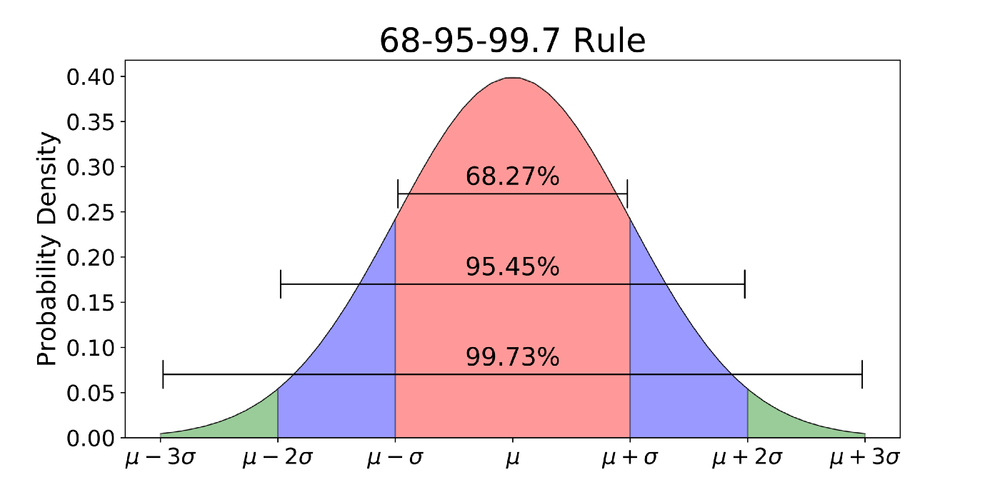
\includegraphics[width=\textwidth]{gaussian.png}
	\captionof{figure}{Regla 68{-}95{-}99.7 para desviación estándar en
		medias de distribuciones gausianas~\cite{galarnyk2018explaining}}\label{fig:fig1}
\end{minipage}
\vspace{1\baselineskip}

La detección de intrusiones es un componente crítico de la detección de anomalías y ha ido evolucionando
significativamente con el paso del tiempo. En la actualidad, los sistemas de detección de intrusiones
se basan en técnicas de aprendizaje automático y de minería de datos, reflejando el progreso de la minería
de excepciones.

El término \textit{detección de anomalías} fue introducido por primera vez por \textit{Patcha y Park} en 2007
~\cite{patcha2007overview}.
